% Importado desde: 2026-03-28_Triada_Variable_y_Fondo_Geometrico_Efectivo.tex
\chapter{Triada variable y fondo geometrico efectivo: --- del protoespacio anisotropo a una geometria emergente lenta}
\label{ch:triada-variable-fondo-geometrico}

\begin{abstract}
Despues de estudiar anisotropias controladas constantes, el paso natural es permitir que los coeficientes efectivos varien lentamente en el protoespacio. Este documento formula, de manera pedagógica y prudente, la idea de una triada efectiva \(e^a{}_i(\vx,n)\) dependiente de la posicion discreta y del tiempo discreto. El objetivo no es derivar todavia una teoria completa de fermiones en espacio curvo, sino mostrar como una variacion lenta del paso microscopico induce un Hamiltoniano de Dirac con coeficientes espaciales variables, y por que eso puede leerse como la primera huella de un fondo geometrico emergente.
\end{abstract}

\section{Pregunta de este paso}
En el capitulo anterior llegamos a un Hamiltoniano anisotropo de la forma
\begin{equation}
H_{\mathrm{aniso}}
=
\tau_z\otimes\left(v_x\sigma_x p_x + v_y\sigma_y p_y + v_z\sigma_z p_z\right)
+ m\,\tau_x\otimes\bbI_2,
\end{equation}
con \(v_x,v_y,v_z\) constantes.

Eso ya permitia una lectura geometrica en terminos de una triada constante. Pero si queremos que el sector Dirac empiece a \enquote{sentir} algo mas parecido a una geometria, el siguiente paso no puede ser seguir con coeficientes constantes: debemos permitir que cambien lentamente de un sitio a otro.

La pregunta central es entonces:
\begin{quote}
\textbf{que pasa si la triada efectiva depende suavemente de la posicion y del tiempo discretos?}
\end{quote}

\section{De triada constante a triada variable}
\subsection{Caso constante}
Recordemos la forma de un bloque de Weyl anisotropo:
\begin{equation}
H_W = \sigma_a\, e^a{}_i\, p_i.
\label{eq:WeylTriadConst}
\end{equation}
En el caso diagonal,
\begin{equation}
e^a{}_i=
\begin{pmatrix}
v_x & 0 & 0\\
0 & v_y & 0\\
0 & 0 & v_z
\end{pmatrix}.
\end{equation}

\subsection{Generalizacion lenta}
Ahora promovemos esos coeficientes a campos lentos:
\begin{equation}
e^a{}_i \longrightarrow e^a{}_i(\vx,n).
\label{eq:triadVariable}
\end{equation}

La palabra \enquote{lento} significa lo siguiente:
\begin{enumerate}[label=\arabic*.]
    \item \(e^a{}_i\) cambia poco entre sitios vecinos;
    \item \(e^a{}_i\) cambia poco entre dos pasos temporales consecutivos;
    \item la longitud de variacion de \(e^a{}_i\) es mucho mayor que la escala de red.
\end{enumerate}

En simbolos, si \(a\) es el espaciamiento espacial y \(\Delta t\) el temporal, suponemos
\begin{equation}
a\,\partial_j e^a{}_i \ll e^a{}_i,
\qquad
\Delta t\,\partial_t e^a{}_i \ll e^a{}_i.
\label{eq:slowvariation}
\end{equation}

\section{Hamiltoniano efectivo local}
\subsection{Idea de aproximacion adiabatica local}
Si la triada varia lentamente, entonces en una pequena region alrededor de un evento \((\vx_0,n_0)\) el sistema se parece mucho a uno con coeficientes constantes iguales a sus valores locales:
\begin{equation}
e^a{}_i(\vx,n)\approx e^a{}_i(\vx_0,n_0).
\end{equation}

Eso sugiere una aproximacion local:
\begin{equation}
H_W^{\mathrm{loc}}(\vx,n)
=
\sigma_a\, e^a{}_i(\vx,n)\, p_i.
\label{eq:localWeyl}
\end{equation}

Al acoplar dos bloques de quiralidad opuesta,
\begin{equation}
H_D^{\mathrm{loc}}(\vx,n)
=
\tau_z\otimes\left(\sigma_a\, e^a{}_i(\vx,n)\, p_i\right)
+m(\vx,n)\,\tau_x\otimes\bbI_2.
\label{eq:localDirac}
\end{equation}

\subsection{Primera interpretacion}
La ecuacion \eqref{eq:localDirac} dice que el fermion efectivo ya no ve el mismo cono en todas partes. El cono local cambia con \(\vx\) y con \(n\).

Esa es la señal estructural que buscabamos:
\begin{quote}
\textbf{la geometria efectiva no esta puesta desde afuera; aparece codificada en la variacion lenta de la regla microscopica.}
\end{quote}

\begin{figure}[h!]
\centering
\begin{tikzpicture}[>=Latex]
  \draw[->] (0,0) -- (6.0,0) node[below] {$x$};
  \draw[->] (0,0) -- (0,3.0) node[left] {$E$};

  \draw[thick,blue!70] (0.7,2.4) -- (1.5,0.0) -- (2.3,2.4);
  \draw[thick,orange!80!black] (2.4,2.4) -- (3.5,0.0) -- (4.6,2.4);
  \draw[thick,green!50!black] (4.5,2.4) -- (5.2,0.0) -- (5.9,2.4);

  \node[blue!70] at (1.5,2.7) {$e^a{}_i(\vx_1)$};
  \node[orange!80!black] at (3.5,2.7) {$e^a{}_i(\vx_2)$};
  \node[green!50!black] at (5.2,2.7) {$e^a{}_i(\vx_3)$};
\end{tikzpicture}
\caption{Interpretacion local: cada region del protoespacio define su propio cono efectivo, ligeramente distinto del de las regiones vecinas.}
\end{figure}

\section{Explicacion paso a paso de por que aparecen terminos extra}
\subsection{Problema de ordenar coeficientes y momentos}
Cuando \(e^a{}_i\) es constante, no importa escribir
\[
e^a{}_i p_i
\quad\text{o}\quad
p_i e^a{}_i.
\]
Pero si \(e^a{}_i=e^a{}_i(\vx)\), eso deja de ser cierto, porque
\begin{equation}
[p_i,f(\vx)] = -\ii\,\partial_i f(\vx).
\end{equation}

Por tanto, al promover coeficientes a funciones del espacio, aparecen automaticamente terminos proporcionales a derivadas de la triada.

\subsection{Ordenamiento simetrico}
La forma mas natural y hermitica del bloque de Weyl es
\begin{equation}
H_W^{\mathrm{sym}}
=
\frac{1}{2}\sigma_a\left(e^a{}_i(\vx)\,p_i + p_i\,e^a{}_i(\vx)\right).
\label{eq:symWeyl}
\end{equation}

Usando \(p_i=-\ii\partial_i\), esto se desarrolla como
\begin{equation}
H_W^{\mathrm{sym}}
=
\sigma_a e^a{}_i(\vx)p_i
-\frac{\ii}{2}\sigma_a \partial_i e^a{}_i(\vx).
\label{eq:extraTerm}
\end{equation}

Aqui aparece ya una novedad crucial:
\begin{quote}
\textbf{una triada variable no solo deforma las velocidades locales; tambien induce terminos adicionales ligados a sus gradientes.}
\end{quote}

\section{Lectura geometrica de los terminos de gradiente}
La ecuacion \eqref{eq:extraTerm} sugiere dos niveles de lectura.

\subsection{Lectura minima}
De la manera mas prudente posible, el termino
\begin{equation}
\Gamma_{\mathrm{eff}}(\vx)
=
-\frac{\ii}{2}\sigma_a\,\partial_i e^a{}_i(\vx)
\end{equation}
puede verse simplemente como una correccion local inducida por la inhomogeneidad del protoespacio.

\subsection{Lectura estructural}
Si damos un paso conceptual adicional, esta clase de terminos recuerda lo que en una formulacion continua mas avanzada aparece como parte de una conexion efectiva para el sector espinorial.

No conviene afirmar todavia que ya derivamos una conexion espinorial completa. Pero si conviene registrar la intuicion correcta:
\begin{quote}
\textbf{cuando la triada varía, el fermion efectivo no siente solo un cono local, sino tambien como ese cono gira o cambia de una region a otra.}
\end{quote}

\section{Dispersion local y metrica efectiva}
En cada punto donde la variacion es suficientemente lenta, podemos congelar \(e^a{}_i(\vx,n)\) y escribir localmente
\begin{equation}
E^2(\vx,\vp)
=
g_{\mathrm{eff}}^{ij}(\vx,n)\,p_i p_j + m^2(\vx,n),
\end{equation}
donde
\begin{equation}
g_{\mathrm{eff}}^{ij}(\vx,n)
=
\delta^{ab} e^a{}_i(\vx,n)e^b{}_j(\vx,n).
\label{eq:metricVariable}
\end{equation}

La novedad respecto del caso anterior es que ahora
\begin{equation}
g_{\mathrm{eff}}^{ij}
\end{equation}
ya no es una matriz fija: es un campo efectivo lento.

\begin{figure}[h!]
\centering
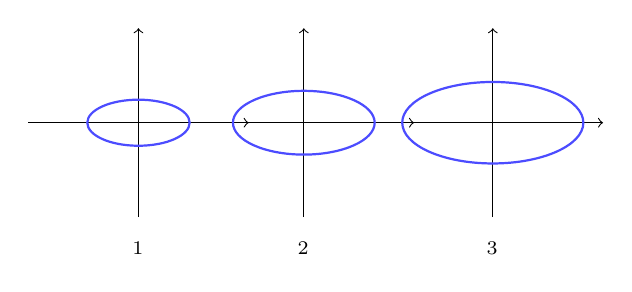
\begin{tikzpicture}[scale=1.0]
  \foreach \x/\r in {0/0.65, 2.1/0.9, 4.5/1.15} {
    \begin{scope}[xshift=\x cm]
      \pgfmathsetmacro{\ry}{0.45*\r}
      \draw[->] (-1.4,0) -- (1.4,0);
      \draw[->] (0,-1.2) -- (0,1.2);
      \draw[thick,blue!70] (0,0) ellipse [x radius=\r, y radius=\ry];
    \end{scope}
  }
  \node at (0,-1.6) {$\vx_1$};
  \node at (2.1,-1.6) {$\vx_2$};
  \node at (4.5,-1.6) {$\vx_3$};
\end{tikzpicture}
\caption{Las superficies locales de energia constante cambian lentamente de una region a otra.}
\end{figure}

\section{Por que este paso es importante para el proyecto}
Este paso es importante por varias razones.

\begin{enumerate}[label=\arabic*.]
    \item Pasa de una geometria efectiva fija a una geometria efectiva variable.
    \item Hace visible la diferencia entre \enquote{una red regular con anisotropia} y \enquote{un protoespacio con textura propia}.
    \item Introduce de manera natural terminos de gradiente que no estaban presentes en el caso homogeneo.
    \item Acerca el programa a la intuicion de un fondo geometrico sin exigir todavia toda la maquinaria de espacio-tiempo curvo.
\end{enumerate}

\section{Que se preserva y que cambia}
\subsection{Lo que se preserva}
Mientras la variacion sea lenta y la triada sea invertible en cada region,
\begin{enumerate}[label=\arabic*.]
    \item el sector infrarrojo sigue siendo localmente tipo Dirac;
    \item la estructura de Clifford sigue organizada por la fibra interna;
    \item la dispersion sigue siendo lineal a escalas suficientemente grandes.
\end{enumerate}

\subsection{Lo que cambia}
Pero ahora cambian varias cosas:
\begin{enumerate}[label=\arabic*.]
    \item la isotropia local puede variar de punto a punto;
    \item aparecen terminos asociados a gradientes de la triada;
    \item la interpretacion ya no es la de un cono unico global, sino la de una familia de conos locales.
\end{enumerate}

\section{Lectura prudente en lenguaje de protoespacio}
La leccion conceptual puede resumirse asi:
\begin{quote}
\textbf{un protoespacio no necesita producir una sola ecuacion de Dirac con coeficientes constantes; puede producir una familia local de ecuaciones de Dirac cuyas variaciones lentas codifican su estructura interna.}
\end{quote}

Eso es muy cercano a lo que queriamos desde el comienzo: que la fisica infrarroja no sea solo un accidente espectral, sino una ventana hacia la organizacion microscopica del sustrato discreto.

\section{Siguiente paso natural}
Desde aqui hay dos continuaciones especialmente prometedoras:
\begin{enumerate}[label=\arabic*.]
    \item estudiar un ejemplo concreto de triada variable, por ejemplo una anisotropia que cambie solo a lo largo de una direccion;
    \item comparar esta construccion con la forma estandar de la ecuacion de Dirac en un fondo con triadas y conexion espinorial.
\end{enumerate}

La primera ruta parece la mejor para seguir construyendo intuicion sin cargar aun demasiada formalidad.

\section*{Conclusion}
El resultado central de este capitulo es el siguiente:
\begin{quote}
\textbf{si la triada efectiva del protoespacio varía lentamente, el sector Dirac no desaparece; se vuelve local, y sus coeficientes pasan a codificar una geometria efectiva dependiente del lugar y del tiempo.}
\end{quote}

Ese es el primer paso serio hacia una lectura geométrica mas rica del protoespacio, sin perder el control matematico del programa.
